%SourceDoc ../YourName-Dissertation.tex
% \vspace*{-80mm}
\chapter{Background} \label{chapter1:Background}

\section{\sloppy Gaussian Processes}

Consider a \emph{spatial stochastic process}~\cite{gelfand2010handbook}, a collection of variables $\{Y(\bm{s}): \bm{s} \in \mathcal{D} \subseteq \mathbb{R}^d\}$ that vary over some continuous spatial domain $\mathcal{D}$. In most applications the dimension is $d = 2$ or $d = 3$; the novel method presented here is valid for any $d$, but applications focus on the $d = 2$ case. If we fix a particular finite set of spatial locations $\{\bm{s}_1, \dots, \bm{s}_n\} \subset \mathcal{D}$, then
\begin{equation}
(Y(\bm{s}_1), \dots, Y(\bm{s}_n))^T
\end{equation}
is a random vector where each element is associated with one location. The multivariate distribution of this random vector contains information about the spatial dependencies between all $n$ locations.

We can specify the distribution of the entire process $\{Y(\bm{s})\}$ as the collection of all finite-dimensional joint distributions
\begin{equation} \label{eq:joint}
F(y_1, \dots, y_n; \bm{s}_1, \dots, \bm{s}_n) = P(Y(\bm{s}_1) \leq y_1, \dots, Y(\bm{s}_n) \leq y_n)
\end{equation}
for every value of $n$ and every set of $n$ spatial locations in $\mathcal{D}$. A \emph{Gaussian process} is a special case in which every distribution in \eqref{eq:joint} is multivariate normal~\cite{gelfand2010handbook}. As a result, the distributions are all completely characterized by their means and covariance matrices, which makes Gaussian processes much easier to work with than non-Gaussian spatial stochastic processes.

% section gaussian_processes (end)

\section{Stationarity and Isotropy} % (fold)
\label{sec:stationarity_and_isotropy}

Throughout this work we will be making two key assumptions: Gaussian processes are \emph{stationary} and \emph{isotropic}. A stationary Gaussian process is one that does not vary with spatial shifts. That is,
\[
E[Y(\bm{s})] = E[Y(\bm{s} + \bm{h})] = \bm{\mu}
\]
and
\[
\textrm{Cov}(Y(\bm{s}), Y(\bm{s} + \bm{h})) = \textrm{Cov}(Y(\bm{0}), Y(\bm{h})) = C(\bm{h}).
\]
Here $C(\bm{h}), \bm{h} \in \mathbb{R}^d$ is called the \emph{covariance function}.

In an isotropic Gaussian process, the covariance function depends on $\bm{h}$, the vector separating two locations, only through the distance $||\bm{h}||$ between them. In this setting, we can express the covariance function simply as $C: [0, \infty) \to \mathbb{R}$. If we assume without loss of generality that the process is standardized, we can further claim that $C(0) = 1$.

Define $\mathcal{C}_d$ as the set of all continuous isotropic covariance functions in $d$ dimensions. Further define $\mathcal{C}_\infty = \bigcap_{d=1}^\infty \mathcal{C}_d$ as the set of all functions that are valid isotropic covariance functions in \emph{all} dimensions. It can be shown~\cite{Stein1999}~\cite{schoenberg1938metric} that
\[
	\mathcal{C}_1 \supseteq \mathcal{C}_2 \supseteq \cdots \supseteq \mathcal{C}_\infty
\]
and that a function $C(h)$ is in $\mathcal{C}_\infty$ if and only if it can be written in the form
\[
	C(h) = \int_0^\infty \exp(-h^2u^2) \; dG(u)
\]
for some $G$ bounded and non-decreasing on $[0, \infty)$~\cite{Stein1999}.

% section stationarity_and_isotropy (end)

\section{Covariance Function Estimation} % (fold)
\label{sec:covariance_function_estimation}

Due to the Gaussian nature of the joint distributions, Gaussian processes are completely characterized by their mean (which without loss of generality we can assume to be 0) and their covariance function. Unsurprisingly, therefore, estimating $C$ given some observations $\{y_1, \dots, y_n\}$ is of great interest. Unfortunately, not just any estimate will produce a valid Gaussian process. $C$ must be a \emph{positive definite function}, which means that for any $n$ and any $\{\bm{s}_1, \dots, \bm{s}_n\} \in \mathcal{D}$, the joint distribution of $\{Y(\bm{s}_1), \dots, Y(\bm{s}_n)\}$ must have a non-negative definite covariance matrix. It is easy to see why this restriction is necessary; by definition $\{Y(\bm{s}_1), \dots, Y(\bm{s}_n)\}$ are jointly normally distributed, so their covariance matrix had better be valid. However, this turns out to be a strong restriction, and it is very difficult to directly estimate $C$ in such a way that forces positive definiteness.

To overcome this, one classical approach~\cite{gelfand2010handbook} is to select a parametric family of covariance functions that are known to be positive definite and estimate the parameters using restricted maximum likelihood (REML) or some other method. A popular choice of parametric families is the \emph{Mat\'{e}rn} class of functions~\cite{handcock1994approach}, which take the form
\begin{equation} \label{eq:matern}
C(h) = \frac{\sigma}{2^{\nu - 1}\Gamma(\nu)} \left( \frac{2\nu^{1/2}h}{\rho} \right)^{\nu} \mathcal{K}_{\nu} \left( \frac{2\nu^{1/2}h}{\rho} \right), \qquad \sigma, \nu, \rho > 0.
\end{equation}
Here $\mathcal{K}_\nu$ is a modified Bessel function of the third kind. It can be shown~\cite{Stein1999} that all functions in this class belong to $\mathcal{C}_\infty$. Some examples of Mat\`ern covariance functions are shown in Figure~\ref{fig:matern_examples}.


\begin{figure}[!htb]
	\centering
	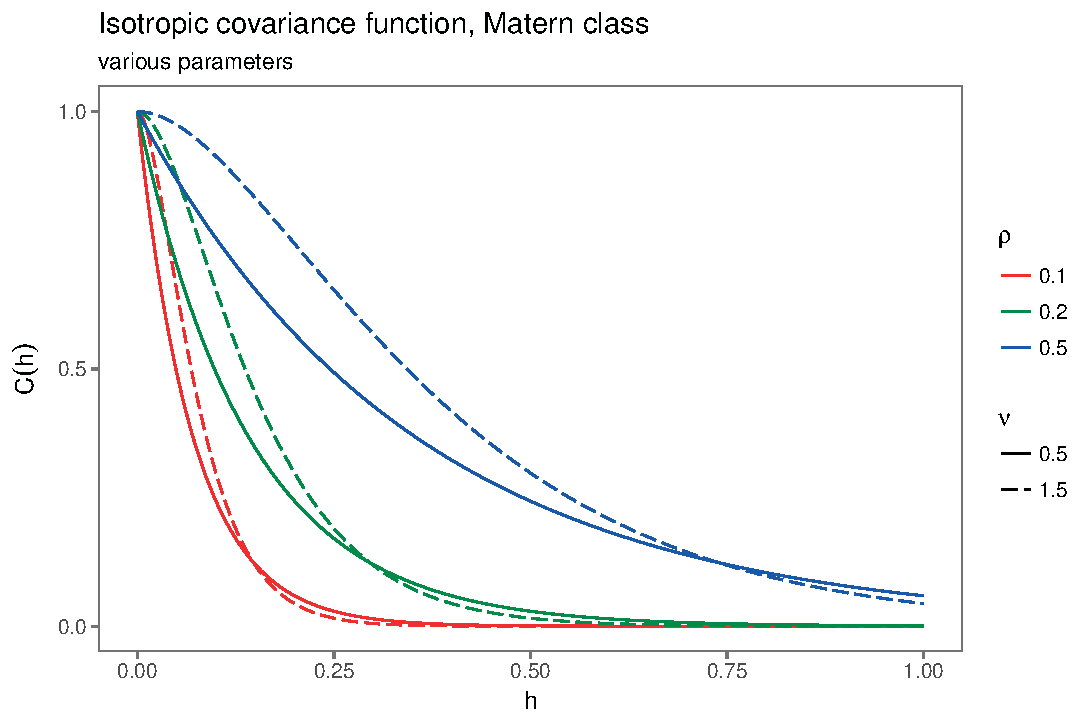
\includegraphics[width=0.95\textwidth]{matern_examples.pdf}
	\caption{\small The Mat\`ern isotropic covariance function \eqref{eq:matern} for various choices of $\nu$ and $\rho$.}
	\label{fig:matern_examples}
\end{figure}


Another notable family is the \emph{exponentially damped cosine} class. 
\begin{equation} \label{eq:dampedcos}
	C(h) = \exp \left( -\tau \frac{h}{\theta} \right) \cos \left( \frac{h}{\theta} \right), \qquad \tau \geq \frac{1}{\tan \frac{\pi}{2d}}, \quad \theta > 0.
\end{equation}
Unlike the Mat\`ern class, the damped cosine class allows for negative correlations at certain distances. This non-monotonic behavior is known in geostatistical applications~\cite{Ye2015} as a \emph{hole effect}, and can be seen in Figure~\ref{fig:dampedcos_examples}. The restriction on $\tau$ that depends on $d$ is necessary for functions of this form to be included in $\mathcal{C}_d$~\cite{gelfand2010handbook}. Note, however, that $\tan(\pi/2d) \to 0$ as $d \to \infty$, so this set of functions is not a member of $\mathcal{C}_\infty$. The damped cosine family is more flexible in some sense than the Mat\`ern family, because it allows for some periodic behavior as well as negative correlations that a Mat\`ern function would not be able to capture. However, as Michael Stein points out~\cite{Stein1999}, the advantage of the Mat\`ern family is that the smoothness of the process, i.e. the degree of differentiability, is captured by the $\nu$ parameter and can be estimated from the data. The smoothness is closely related to the local behavior of the process, and so being able to estimate it is crucial to obtaining good performance when interpolating the process at new locations.

\begin{figure}[!htb]
	\centering
	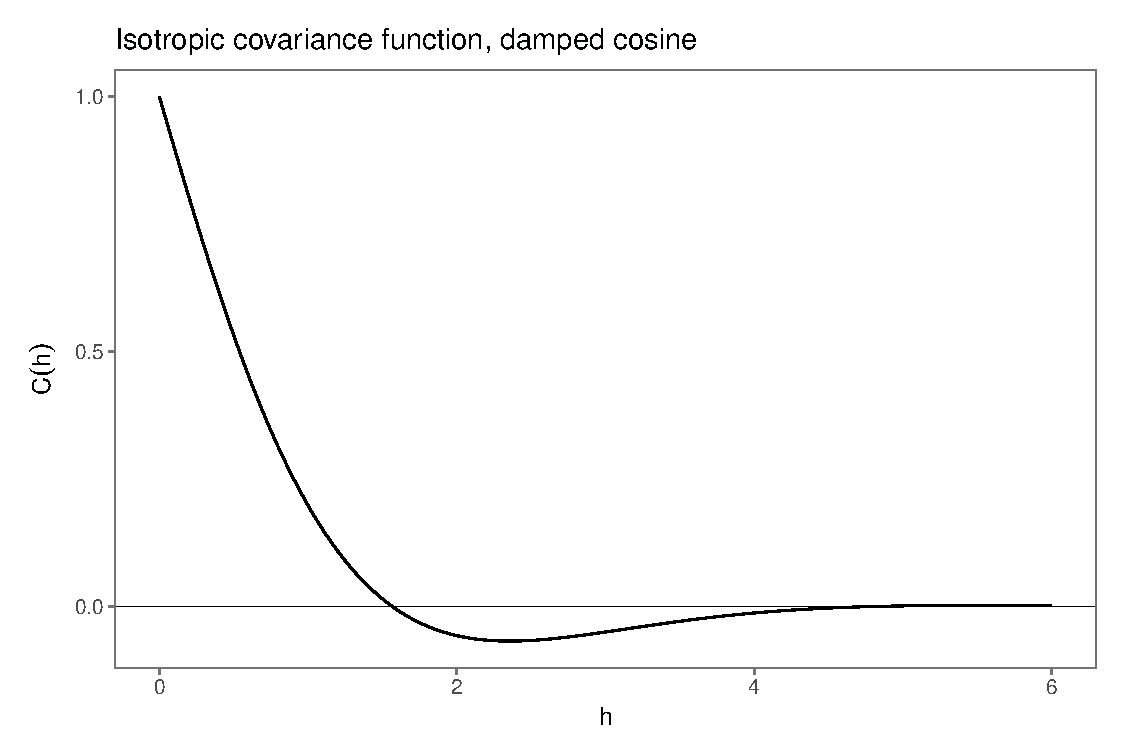
\includegraphics[width=0.95\textwidth]{dampedcos_examples.eps}
	\caption{\small The damped cosine isotropic covariance function \eqref{eq:dampedcos} for $\tau = 1$. Notice that $C(h) < 0$ for certain values of $h$.}
	\label{fig:dampedcos_examples}
\end{figure}

The method of fitting the data to a parametric family of covariance functions can produce a good estimate if the true covariance structure is close to the structure assumed by the choice of parametric family. However, there is no guarantee that this will be the case. For instance, if the true covariance contains a hole effect, there is no way for a Mat\`ern model to capture it since $C(h) > 0$ for all $h$. More preferable would be a semiparametric Bayesian method that allows the spatial dependence in the data itself to determine the shape of $C$, and not the choice of parametric family.

% subsection estimating_the_covariance_function (end)

\section{The Spectral Domain and Bochner's Theorem} % (fold)
\label{sec:bochner_s_theorem}

The method proposed in this work takes advantage of the following result from Bochner~\cite{bochner1955harmonic}. A real-valued continuous function $C$ is positive definite if and only if it is the Fourier transform of a symmetric, non-negative, finite measure $F$ on $\mathbb{R}^d$. That is, $C$ is positive definite if and only if
\begin{equation} \label{eq:bochner}
C(\bm{h}) = \int_{\mathbb{R}^d} \exp(i \bm{h}^T \bm{\omega}) \; dF(\bm{\omega}) = \int_{\mathbb{R}^d} \cos(\bm{h}^T \bm{\omega}) \; dF(\bm{\omega}).
\end{equation}
The imaginary part of the above integral drops out because $F$ is symmetric. Usually this measure has a Lebesgue density, $f$, which is referred to as the \emph{spectral density}~\cite{gelfand2010handbook}. Then \eqref{eq:bochner} becomes
\[
C(\bm{h}) = \int_{\mathbb{R}^d} \cos(\bm{h}^T \bm{\omega}) \; f(\bm{\omega}) \; d\bm{\omega}.
\]
Because we are operating under the assumption that the Gaussian process described by $C$ is isotropic, $C$ is a function of a scalar $h$, not a vector:
\begin{equation} \label{eq:bochner2}
C(h) = \int_{\mathbb{R}} \cos(h\omega) \; f(\omega) \; d\omega.
\end{equation}
The relationship between the covariance function and the spectral density given in \eqref{eq:bochner2} gives us an alternative way to estimate $C$. If we can estimate the spectral density such that we ensure it is a valid symmetric density, then we are assured that $C$ is positive definite.

There have been some proposals for non- and semi-parametric methods that estimate $C$ using the spectral domain. Most notably, Im, Stein, and Zhu~\cite{IM2007} estimate the spectral density using a combination of cubic B-splines with an explicitly estimated algebraically decaying tail. They use the fact that when we assume isotropy, \eqref{eq:bochner} can be written as an integral over only one dimension:
\[
	C(h) = 2^{(d-2)/2}\Gamma(d/2) \int_0^\infty (hu)^{-(d-2)/2} J_{(d-2)/2}(hu) \; dG(u)
\]
where $J_\nu(\cdot)$ is the Bessel function of the first kind of order $\nu$. Once the spectral density has been estimated, they are assured that the resulting covariance function is positive definite, and then can find the values of the parameters that maximize the likelihood of their data. Our method follows this same concept, with some notable differences outlined in Chapter~\ref{chapter2:Procedure}.

Another, earlier method was put forth by Hall, Fisher and Hoffmann~\cite{Hall1994}. They proposed a multistep process which begins with a kernel estimate of the covariogram. Because the kernel estimate is not necessarily positive definite, they find its Fourier transform, set all frequencies above the first negative value to zero, and then Fourier transform it back to the spatial domain. In the simulation study in Chapter~\ref{chapter3:Simulation-Study} we compare our method to the one from Hall et al., as well as to the Mat\`ern model fit by maximum likelihood.

In Chapter~\ref{chapter4:Data-Application}, we apply our method to data from [wherever it's from]. The results are discussed in Chapter~\ref{chapter5:Conclusions}, as well as possibilities for improvements and future directions to take with this work.

% section bochner_s_theorem (end)
